% Build with XeLaTeX; all lettering uses Arial.
\documentclass[tikz,border=5mm]{standalone}
\usepackage{fontspec}
\setmainfont{Arial}
\setsansfont{Arial}
\usetikzlibrary{arrows.meta}

% Matplotlib tab10 palette.
\definecolor{mplBlue}{HTML}{1F77B4}
\definecolor{mplOrange}{HTML}{FF7F0E}
\definecolor{mplGreen}{HTML}{2CA02C}
\definecolor{mplGray}{HTML}{7F7F7F}

\begin{document}
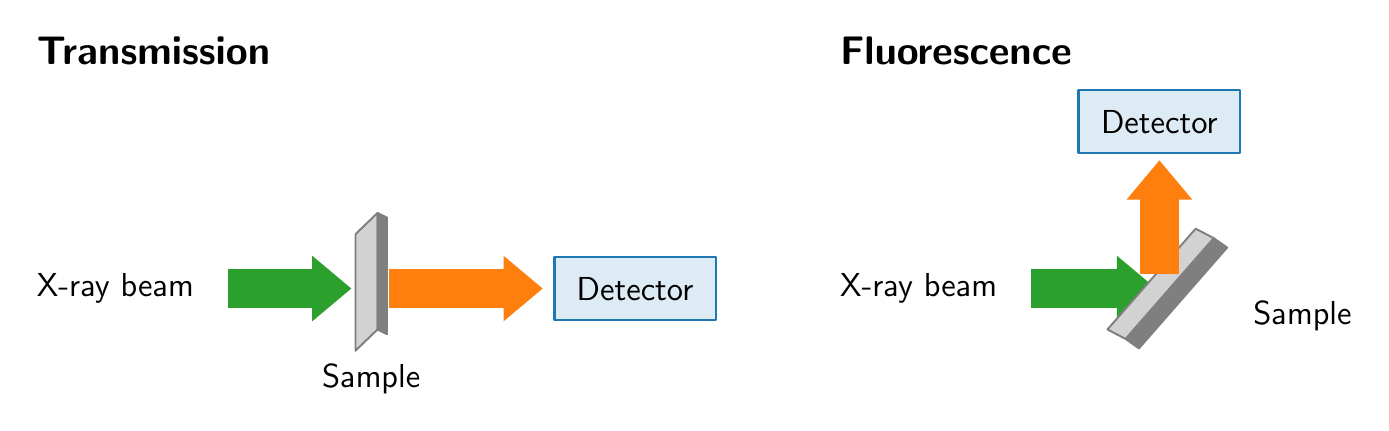
\begin{tikzpicture}[
  x=1cm,y=1cm,
  font=\sffamily\fontsize{12}{14}\selectfont,
  line join=round,
  heading/.style={anchor=west,font=\sffamily\bfseries\fontsize{15}{18}\selectfont},
  detector/.style={draw=mplBlue,fill=mplBlue!15,line width=.9pt,
    minimum width=2.05cm,minimum height=.8cm,inner sep=3pt},
  beam/.style={line width=5mm,-{Triangle[length=5mm,width=8mm]},line cap=butt}
]
% Transmission: incident beam, planar sample, transmitted beam, detector.
\node[heading] at (0,3.02) {Transmission};
\node[anchor=west] at (0,0) {X-ray beam};
\draw[beam,mplGreen] (2.55,0) -- (4.12,0);
\path[fill=mplGray!35,draw=mplGray,line width=.7pt]
  (4.17,-.79) -- (4.45,-.52) -- (4.45,.96) -- (4.17,.69) -- cycle;
\path[fill=mplGray,draw=mplGray,line width=.7pt]
  (4.45,-.52) -- (4.57,-.58) -- (4.57,.90) -- (4.45,.96) -- cycle;
\draw[beam,mplOrange] (4.59,0) -- (6.55,0);
\node[detector,anchor=west] at (6.68,0) {Detector};
\node at (4.37,-1.15) {Sample};

% Fluorescence: sample at 45 degrees, detector at 90 degrees to incidence.
\begin{scope}[xshift=10.2cm]
  \node[heading] at (0,3.02) {Fluorescence};
  \node[anchor=west] at (0,0) {X-ray beam};
  \draw[beam,mplGreen] (2.55,0) -- (4.14,0);
  \path[fill=mplGray,draw=mplGray,line width=.7pt]
    (3.75,-.64) -- (3.92,-.76) -- (5.04,.52) -- (4.87,.64) -- cycle;
  \path[fill=mplGray!35,draw=mplGray,line width=.7pt]
    (3.75,-.64) -- (4.87,.64) -- (4.64,.76) -- (3.52,-.52) -- cycle;
  \draw[beam,mplOrange] (4.18,.18) -- (4.18,1.63);
  \node[detector] at (4.18,2.12) {Detector};
  \node[anchor=west] at (5.25,-.35) {Sample};
\end{scope}
\end{tikzpicture}
\end{document}
